\scanpage{127}
\uline{Lemme 3}\quad
Soit \(f:X\mathbin{\text{---}}Y\) un morphisme
\inserted{compactifiable} de type fini, de dim relative \(\le d'\),
\(F\) un \(\unsure{Z_l|Q_l}\)-faisceau admissible de type \(\le d\) sur \(X\),
alors pour \deleted{\unsure{tout}} \(i\), \(R^i_!f(F)\) sur \(Y\)
sont admissibles de type \(\le d+d'\).
\figure{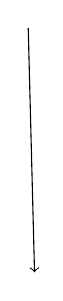
\begin{tikzpicture}\draw[->] (0,3.1)--(.08,0);\end{tikzpicture}}

On peut supposer \(Y=\operatorname{Sp}k\), \(k\) un corps.

Récurrence sur \(d+d'\), trivial si \(d'\le0\).
Supposons \(d+d'>0\), et le th. démontré pour les
\deleted{\unsure{d'}} \inserted{\(\delta'<d'\)}.

Soit \(U\subset X\) \inserted{ouvert} lisse sur \(k\) et dense dans \(X\),
et \inserted{que \(F|U\) ait une filtration \(d\)-admissible.}
[N.B. on est obligé dans la déf. plus haut d'admettre une extension radicielle sur la base.]
et soit \(Z=X-U\).

On a
\[
R^n_!f_U(F|U)\longrightarrow R^n_!f_*(F)
\mathbin{\text{---}} R^n_!f_{\unsure{Z}*}(F|\unsure{Y|Z})
\]
ce qui nous ramène au cas de \(f_Z\) et \(f_U\) grâce aux lemmes 1 et 2;
le cas de \(f_Z\) est connu par l'hyp. de réc.,
et \deleted{alors} \unsure{pour le cas où} \(X\) est lisse
sur \(k\) et a une filtration \(d\)-admissible.

Par dévissage et le lemme \(1\unsure{a|er}\) on peut supposer que \(F\)
est un quotient \inserted{\unsure{ess. const.}} d'un
% archive foliation: 126
